\documentclass[letterpaper,12pt,fleqn]{article}
\usepackage{matharticle}
\pagestyle{empty}
\newcommand{\vx}{\vec{x}}
\newcommand{\vy}{\vec{y}}
\newcommand{\vyp}{\vec{y}\,'}
\newcommand{\seg}[1]{\overline{#1}}
\newcommand{\norm}[1]{\left\|#1\right\|}
\begin{document}
\section*{Convex Sets}

\begin{definition}[Line Segment]
  Let $E$ be a vector space and $\vx,\vy\in E$. The \emph{line segment} from
  $\vx$ to $\vy$, denoted $\seg{xy}$, is given by:
  \[\seg{xy}=\{(1-t)x+ty\mid t\in[0,1]\}\]
\end{definition}

\begin{definition}[Convex]
  Let $E$ be a vector space. To say that $S\subset E$ is \emph{convex} means:
  \[\forall\,\vx,\vy\in S,\seg{xy}\subset S\]
\end{definition}

\begin{examples}
  \listbreak
  \begin{enumerate}
  \item Vector spaces
  \item Closed balls
  \item Not convex:

    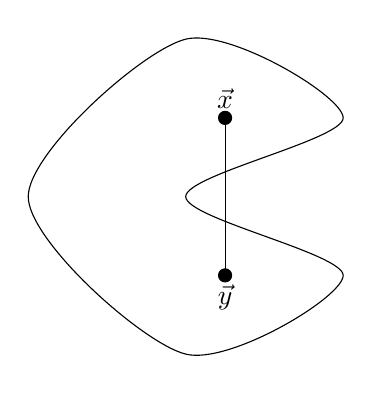
\begin{tikzpicture}
      \draw [smooth cycle] plot coordinates {
        (0,0) (2,-2) (4,-1) (2,0) (4,1) (2,2)
      };
      \node [draw,circle,fill,scale=0.5] (x) at (2.5,1) {};
      \node [above] at (x) {$\vx$};
      \node [draw,circle,fill,scale=0.5] (y) at (2.5,-1) {};
      \node [below] at (y) {$\vy$};
      \draw (x) to (y);
    \end{tikzpicture}
  \end{enumerate}
\end{examples}

\begin{theorem}[Closest Point Property]
  Let $H$ be a Hilbert space and let $S$ be a closed and convex subset of $H$.
  $\forall\,\vx\in H$, there exists a unique closest point $\vy\in S$ to $\vx$:
  \[\exists!\,\vy\in S,d(\vx,S)=\norm{\vx-\vy}=d(x,y)\]
\end{theorem}

\begin{theproof}
  \begin{minipage}{3in}
    Assume $\vx\in H$. \\
    $d(\vx,S)=\inf_{\vy\in S}\norm{\vx-\vy}$ \\
    So $\exists\,(\vy_n)$ in $S$ such that $\norm{\vx-\vy_n}\to d$. \\
  \end{minipage}
  \begin{minipage}{3in}
    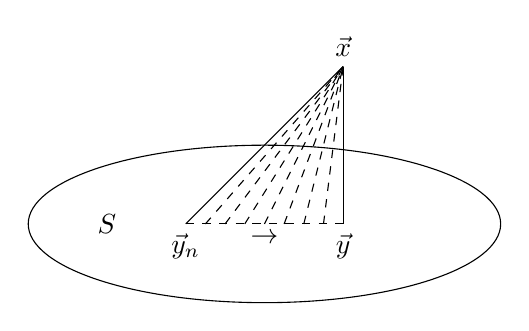
\begin{tikzpicture}
      \draw (0,0) ellipse (3 and 1);
      \node [scale=0.01] (yn) at (-1,0) {};
      \node [below] at (yn) {$\vy_n$};
      \node [scale=0.01] (y) at (1,0) {};
      \node [below] at (y) {$\vy$};
      \node [scale=0.01] (x) at (1,2) {};
      \node [above] at (x) {$\vx$};
      \draw (yn) to (x);
      \draw (y) to (x);
      \draw [dashed] (yn) to node [below] {$\to$} (y);
      \draw [dashed] (-0.75,0) to (x);
      \draw [dashed] (-0.5,0) to (x);
      \draw [dashed] (-0.25,0) to (x);
      \draw [dashed] (0.0,0) to (x);
      \draw [dashed] (0.25,0) to (x);
      \draw [dashed] (0.5,0) to (x);
      \draw [dashed] (0.75,0) to (x);
      \node at (-2,0) {$S$};
    \end{tikzpicture}
  \end{minipage}

  Claim: $(\vy_n)$ is Cauchy.

  \begin{minipage}{3in}
    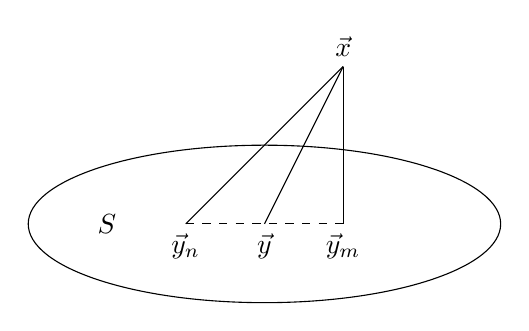
\begin{tikzpicture}
      \draw (0,0) ellipse (3 and 1);
      \node [scale=0.01] (yn) at (-1,0) {};
      \node [below] at (yn) {$\vy_n$};
      \node [scale=0.01] (ym) at (1,0) {};
      \node [below] at (ym) {$\vy_m$};
      \node [scale=0.01] (y) at (0,0) {};
      \node [below] at (y) {$\vy$};
      \node [scale=0.01] (x) at (1,2) {};
      \node [above] at (x) {$\vx$};
      \draw (yn) to (x);
      \draw (ym) to (x);
      \draw (y) to (x);
      \draw [dashed] (yn) to (ym);
      \node at (-2,0) {$S$};
    \end{tikzpicture}
  \end{minipage}
  \begin{minipage}{3in}
    Let $\vy=\frac{\vy_n+\vy_m}{2}$.
    
    Note that $\vy\in S$ because $S$ is convex.
  \end{minipage}

  Apply the parallelogram law with $\vx-\vy_n$ and $\vx-\vy_m$:
  \begin{eqnarray*}
    \norm{(\vx-\vy_n)+(\vx-\vy_m)}^2+\norm{(\vx-\vy_n)-(\vx-\vy_m)}^2 &=&
    2\norm{\vx-\vy_n}^2+2\norm{\vx-\vy_m}^2 \\
    \norm{2\vx-(\vy_m+\vy_n)}^2+\norm{\vy_m-\vy_n}^2 &=&
    2\norm{\vx-\vy_n}^2+2\norm{\vx-\vy_m}^2 \\
    4\norm{\vx-\frac{\vy_m+\vy_n}{2}}^2+\norm{\vy_m-\vy_n}^2 &=&
    2\norm{\vx-\vy_n}^2+2\norm{\vx-\vy_m}^2
  \end{eqnarray*}
  And so:
  \[\norm{\vy_m-\vy_n}^2=2\norm{\vx-\vy_n}^2+2\norm{\vx-\vy_m}^2-
  4\norm{\vx-\frac{\vy_m+\vy_n}{2}}^2\to2d^2+2d^2-4d^2=0\]
  Therefore $(\vy_n)$ is Cauchy.

  Now, $H$ is Hilbert and thus complete, so $\vy_n\to\vy\in H$. \\
  But $S$ is closed, and so $\vy\in S$.

  Therefore such a $\vy\in S$ exists.

  Now, assume that there are two such points: $\vy$ and $\vyp$. \\
  Applying the parallelogram law with $\vx-\vy$ and $\vx-\vyp$:
  \begin{eqnarray*}
    \norm{(\vx-\vy)+(\vx-\vyp)}^2+\norm{(\vx-\vy)-(\vx-\vyp)}^2 &=&
    2\norm{\vx-\vy}^2+2\norm{\vx-\vyp}^2 \\
    \norm{2\vx-(\vyp+\vy)}^2+\norm{\vyp-\vy}^2 &=&
    2\norm{\vx-\vy}^2+2\norm{\vx-\vyp}^2 \\
    4\norm{\vx-\frac{\vyp+\vy}{2}}^2+\norm{\vyp-\vy}^2 &=&
    2\norm{\vx-\vy}^2+2\norm{\vx-\vyp}^2
  \end{eqnarray*}
  And so:
  \[\norm{\vyp-\vy}^2=2\norm{\vx-\vy}^2+2\norm{\vx-\vyp}^2-
  4\norm{\vx-\frac{\vyp+\vy}{2}}^2\le2d^2+2d^2-4d^2=0\]

  Therefore $\vyp-\vy=0$ and thus $\vy=\vyp$, proving uniqueness.
\end{theproof}

\end{document}
